The state estimation of a vehicle sits at the intersection of vehicle dynamics and control theory. Both knowledge of the dynamics of a race car and the algorithms to model their physics in equations and software is required to design a successful solution. Therefore, we explore the fundamentals of vehicle dynamics, estimation algorithms and sensor failure detection in this chapter.

Throughout this thesis, the conventions of ISO 8855~\cite{ISO.2011} will be used, which assumes a right-handed coordinate system. The vehicle coordinate system uses an upward $z$-axis with a forward $x$-axis and a leftward $y$-axis, while the earth-fixed coordinate system uses an upward $z$-axis with an eastward $x$-axis and a northward $y$-axis. The vehicle's\gls{cog} is used as origin/reference point of the vehicle coordinate system. In case of mixed coordinate systems, left-superscript will be used to denote the reference frame (e.g., $\prescript{V}{}{x}$ for vehicle coordinates, $\prescript{E}{}{x}$ for earth-fixed coordinates).



\section{Rigid Body Kinematics}
The fundamental laws of mechanics apply to race cars as they do to any other body. These laws relate, among others, the body's linear and angular position and its time derivatives, resulting in translational and rotational changes. Their three-dimensional vector definitions are shown in Equations \ref{eq:linear-quantities} and \ref{eq:angular-quantities}. To simplify the equations, a rigid body is assumed. This means, that deformations which occur in the vehicle during dynamic maneuvers are negligibly small or vanish. Therefore, points on the body maintain the same distance relative to each other at all times. Furthermore, a two-dimensional motion in the road plane can be assumed in many cases because the effects vertical dynamics are negligible. The simplified equations for that case will also be shown.

\begin{subequations}\label{eq:linear-quantities}
\begin{alignat}{2}%
p &= \begin{bmatrix}x, y, z\end{bmatrix}^T \\%
v &= \begin{bmatrix}v_x, v_y, v_z\end{bmatrix}^T \\%
a &= \begin{bmatrix}a_x, a_y, a_z\end{bmatrix}^T%
\end{alignat}
\end{subequations}
\begin{subequations}\label{eq:angular-quantities}
\begin{alignat}{2}%
\varphi &= \begin{bmatrix}\phi, \theta, \psi\end{bmatrix}^T \\%
\omega &= \begin{bmatrix}\dot{\phi}, \dot{\theta}, \dot{\psi}\end{bmatrix}^T \\%
\alpha &= \begin{bmatrix}\ddot{\phi}, \ddot{\theta}, \ddot{\psi}\end{bmatrix}^T%
\end{alignat}
\end{subequations}

The linear displacement $p$ of a body describes its position relative to the origin of its reference frame. It comprises a longitudinal component along the $x$-axis, a lateral component along the $y$-axis and a vertical component along the $z$-axis. Its first time derivative $v = \frac{dr}{dt}$ and second time derivative $a = \frac{d^2r}{dt^2}$ are the body's linear velocity and acceleration, respectively. \\ The angular orientation $\varphi$ of a body describes its rotation in the reference frame. It can be described by the roll angle $\phi$ around the $x$-axis, the pitch angle $\theta$ around the $y$-axis and the yaw angle $\psi$ around the $z$-axis. The angular velocity $\omega$ and acceleration $\alpha$ describe the element-wise time derivatives of these angles.


\subsection{Transformation of Linear Velocities}
All points on a rigid body experience the same angular velocity, i.e. $\omega^A = \omega^B$ for any two points $A, B$ on that body at all times. However, these two points will generally not have the same linear velocity vector, since it is affected by their location $r$ relative to the \gls{cog}. Only when $\omega = \mathbb{0}$, the linear velocity is equal for all points on the body, i.e. $v^A = v^B$. If there is a non-zero angular velocity, the following holds for any point $P$, assuming the velocity at the \gls{cog} is known (the expanded form can be found in Appendix \ref{sec:appendix-transformation-linvel}):

% For SFII transformation
\begin{equation}\label{eq:offcenter-velocity-3d}%
v^P = v^{CG} + \omega \times r^P%
\end{equation}

This becomes easier to visualize when regarding the two-dimensional case, where $v_z$, $\dot{\phi}$ and $\dot{\theta}$ are disregarded, as shown in Equation \ref{eq:offcenter-velocity-2d}.

\begin{equation}\label{eq:offcenter-velocity-2d}%
v^P%
= \begin{bmatrix}v_x^{CG} \\ v_y^{CG} \\ 0\end{bmatrix} + \begin{bmatrix}0 \\ 0 \\ \dot{\psi}\end{bmatrix} \times \begin{bmatrix}r_x \\ r_y \\ r_z\end{bmatrix}%
= \begin{bmatrix}v_x^{CG} \\ v_y^{CG} \\ 0\end{bmatrix} + \begin{bmatrix}-\dot{\psi} \cdot r_y \\ \dot{\psi} \cdot r_x \\ 0\end{bmatrix}%
 \end{equation}

Let us regard the example scenario shown in Figure \ref{fig:offcenter-velocity}, where the vehicle has a positive yaw rate and the \gls{cog} is moving forward and to the left. Point $A$ is at the front left ($r_x > 0$, $r_y > 0$), while point $B$ is at the rear right ($r_x < 0$, $r_y < 0$). Since $r$ is defined relative to the \gls{cog}, its position is $\mathbb{0}$. Due to the positive yaw rate, $A$ experiences a higher $v_y$ but lower $v_x$ than the \gls{cog}. $B$, on the other hand, experiences a higher $v_x$ but lower $v_y$ than the \gls{cog}. If the yaw rate were zero, all points would experience the same linear velocity.

\begin{figure}
	\centering
	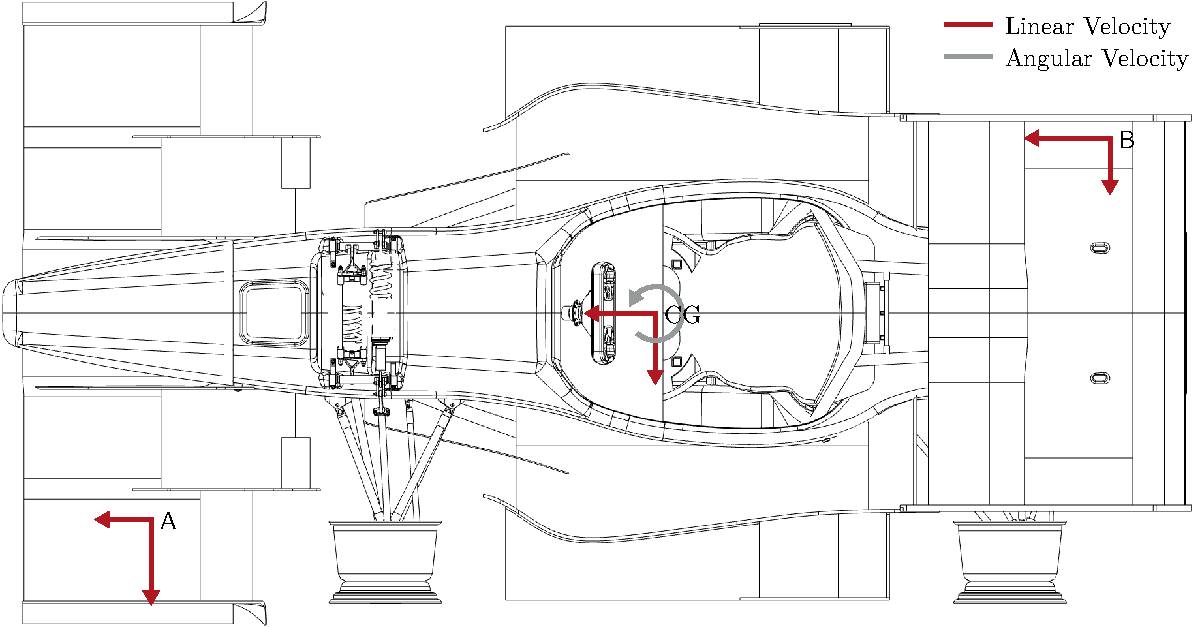
\includegraphics[width=\textwidth]{offcenter_velocity}%
	\caption{Experienced velocities at off-center points}
	\label{fig:offcenter-velocity}
\end{figure}


\subsection{Transformation of Linear Accelerations}
Like the angular velocity, the angular acceleration is the same at every point on a rigid body, i.e. $\alpha^A = \alpha^B$ for any two points $A, B$ on that body. However, these two points will generally not experience the same linear acceleration. Only if the rotational motion components $\omega$ and $\alpha$ are $\mathbb{0}$, the linear acceleration is equal for all points on the body, i.e. $a^A = a^B$. In the general case, the following holds for any point $P$ at location $r$ (the expanded form can be found in Appendix \ref{sec:appendix-transformation-linacc}):

\begin{equation}\label{eq:offcenter-acceleration-3d}%
a^P = a^{CG} + \alpha \times r^P + \omega \times (\omega \times r^P)%
\end{equation}

We can identify two additional components which affect the experienced linear acceleration. The term $\alpha \times r$ is the tangential acceleration along the circular path around the center of rotation, which is $a_{tan} = \alpha \cdot r$ in scalar notation. More significant due to the squared angular velocity, however, is the introduction of the centripetal acceleration $a_c$ in the term $\omega \times (\omega \times r)$. This term is the vector-equivalent of the acceleration resulting from the centripetal force $F_c$ in Equation \ref{eq:centripetal-acceleration}.

\begin{equation}\label{eq:centripetal-acceleration}%
F_c = \frac{mv^2}{r} \iff a_c = \frac{v^2}{r} = \omega^2 r%
\end{equation}

The two-dimensional form, shown in Equation \ref{eq:offcenter-acceleration-2d}, is more intuitive than its three-dimensional counterpart. Here, $a_z$, $\dot{\phi}$, $\dot{\theta}$, $\ddot{\phi}$ and $\ddot{\theta}$ are assumed to be zero. The inward-direction of the centripetal effect can be seen by the negative signs of the angular velocity part.

\begin{equation}\label{eq:offcenter-acceleration-2d}%
a^P%
= \begin{bmatrix}a_x^{CG} \\ a_y^{CG} \\ 0\end{bmatrix}%
+ \begin{bmatrix}0 \\0 \\ \ddot{\psi}\end{bmatrix} \times \begin{bmatrix}r_x \\ r_y \\ r_z\end{bmatrix} \\%
+ \begin{bmatrix}0 \\ 0 \\ \dot{\psi}\end{bmatrix} \times \left(\begin{bmatrix}0 \\ 0 \\ \dot{\psi}\end{bmatrix} \times \begin{bmatrix}r_x \\ r_y \\ r_z\end{bmatrix}\right)%
= \begin{bmatrix}a_x^{CG} \\ a_y^{CG} \\ 0\end{bmatrix}%
+ \begin{bmatrix}-\ddot{\psi} \cdot r_y \\ \ddot{\psi} \cdot r_x \\ 0\end{bmatrix}%
+ \begin{bmatrix}-\dot{\psi}^2 \cdot r_x \\ -\dot{\psi}^2 \cdot r_y \\ 0\end{bmatrix}%
\end{equation}

We demonstrate these effects in the example scenario shown in Figure \ref{fig:offcenter-acceleration}, which is similar to the one in the previous subsection, but with an additional positive yaw acceleration. In point $A$, the tangential and centripetal acceleration cancel out and even surpass the linear acceleration experienced in the \gls{cog}, resulting in a negative $a_x$ and a much lower $a_y$. The opposite effect occurs in point $B$, where both $a_x$ and $a_y$ are amplified.

\begin{figure}
	\centering
	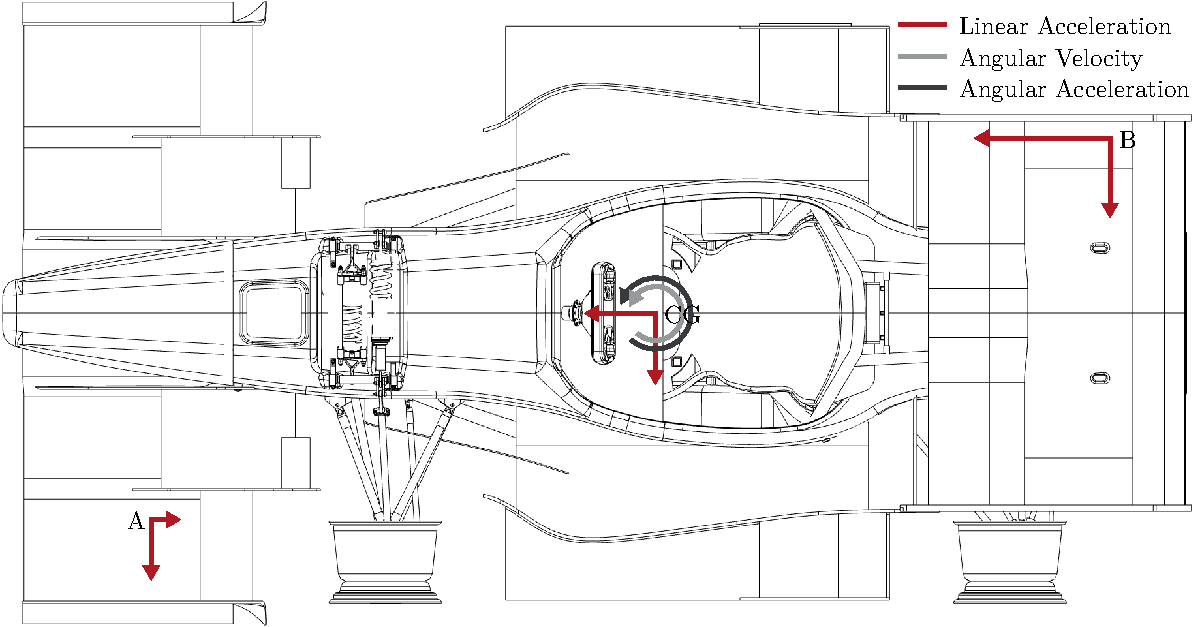
\includegraphics[width=\textwidth]{offcenter_acceleration}%
	\caption{Experienced acceleration at off-center points}
	\label{fig:offcenter-acceleration}
\end{figure}


\subsection{Calculate Angular Acceleration from Linear Acceleration}
Direct measurement of the angular acceleration is often not possible. However, individual components of $\alpha$ can be calculated with two known linear acceleration vectors from different points with known locations $r^A, r^B$ using Equation \ref{eq:angacc-from-linacc-3d}. It is derived from Equation \ref{eq:offcenter-acceleration-3d}, but $a^{CG}$ is cancelled out by the difference while the centripetal acceleration points only towards the center of rotation. The points must not be on the rotation axis, otherwise they experience no angular acceleration. Thus, three non-collinear points are required to determine all components of $\alpha$. While the inverse of a cross product is not uniquely determined as can be seen by the scalar factor $t$, $t = 0$ works well in practice, so this part can be omitted.

% TODO only works if points are not on rotation axis

\begin{equation}\label{eq:angacc-from-linacc-3d}%
a^A - a^B = \alpha \times (r^A - r^B) \implies \alpha = \frac{(r^A - r^B) \times (a^A - a^B)}{\norm{r^A - r^B}^2} + t \cdot (r^A - r^B), t \in \mathbb{R}%
\end{equation}

In two dimensions, this becomes easier to understand. Calculation of the yaw acceleration from the longitudinal and lateral accelerations of two points is shown in Equation \ref{eq:angacc-from-linacc-2d} with $\Delta r = r^A - r^B$ and $\Delta a = a^A - a^B$. When $A$ and $B$ are directly in front of and behind the \gls{cog} on the $x$-axis, $\ddot{\psi} = \frac{\Delta a_y}{\Delta r_x}$.

\begin{equation}\label{eq:angacc-from-linacc-2d}%
\alpha%
= \frac{\begin{bmatrix}\Delta r_x \\ \Delta r_y \\ 0\end{bmatrix} \times \begin{bmatrix}\Delta a_x \\ \Delta a_y \\ 0\end{bmatrix}}{\begin{Vmatrix}\Delta r_x \\ \Delta r_y \\ 0\end{Vmatrix}^2}%
\implies \ddot{\psi} = \frac{\Delta a_y \Delta r_x - \Delta a_x \Delta r_y}{\Delta r_x^2 + \Delta r_y^2}%
\end{equation}


\subsection{Transformation Between Coordinate Systems}
Equations \ref{eq:linear-quantities} and \ref{eq:angular-quantities} use earth-fixed coordinates. Apart from a \gls{gnss}, measurements will be made in vehicle coordinates, however. Therefore, we need equations to transform between these two coordinate system for a point $P$.

% For EKF position--velocity
\begin{equation}%
\prescript{V}{}{v}^P = \prescript{E}{}{v}^P + R \cdot \omega%
\end{equation}




motion equations
wheels to speed



\section{Estimation Algorithms}
goal: solve filtering problem and fuse sensors to obtain optimal state estimate

http://www.anuncommonlab.com/articles/how-kalman-filters-work/index.html
Estimation algorithms
particle filter
kalman filter
EFK
compare

Define residual
disable measurements using separate mask



\section{Failure Detection}
causes: missing connection, no feature correlation for sfii, electromagnetic interference

outlier types: persistent, transient~\cite[p.~170~ff.]{Himmelblau.1994}
outlier, drift, null~\cite[p.~19 f.]{Kabzan.13.05.2019}
transient is easier to detect
separate mechanisms

statistical methods

transient: range and

EKF bank
